\documentclass{homework}
\usepackage{xcolor}
\usepackage{nicematrix}
\usepackage{booktabs}
\usepackage{enumitem}
\usepackage{caption}
\usepackage{subcaption}
\usepackage{leftidx}
\usepackage{tikz}

\NiceMatrixOptions{cell-space-limits = 1pt}

\title{Solutions Excercise 4}
\author{
  Maksimov, Dmitrii\\
  \texttt{dmitrii.maksimov@fau.de} \\
  \texttt{ko65beyp}
  \and
  Ilia, Dudnik\\
  \texttt{ilia.dudnik@fau.de}\\
  \texttt{ex69ahum}
}

\begin{document}

\maketitle

\exercise
Show: if $P=\{x\in \R | Ax\leq b\}$ is a non-empty polyhedron and $I=eq(P)$, then we have: \[aff(P)=\{x\in \R^n|A_{I\cdot}x=b_I\}\]

By definition: \[aff(S)\coloneqq \left\{\sum_{i=1}^t \lambda_i a_i:t\geq 1\text{ and finite}, a_1, \dots, a_t \in S, \lambda_1, \dots, \lambda_t \in \R, \sum_{i=1}^t \lambda_i = 1\right\} \]
Let $\overline{x} \in aff(P),$ then:
\begin{align*}
	&\overline{x} = \lambda_1 x^1 + \dots + \lambda_t x^t \text{ for some } x^1, \dots, x^t \in P, \lambda_1, \dots, \lambda_t \in \R, \sum_{i=1}^t \lambda_i=1 \Rightarrow\\
	&A\overline{x}=\lambda_1 Ax^1+\dots + \lambda_t Ax^t = \left(\sum_{i=1}^t\lambda_i\right)b=b\Rightarrow\\
	&\overline{x} \in \{x:Ax=b\} \Rightarrow aff(P)=\{x\in \R^n|A_{I\cdot}x=b_I\}
\end{align*}

\exercise
Prove or disprove:
\begin{enumerate}[label=(\alph*)]
	\item Let $K$ be a cone. Then $x+y\in K$ holds fo all $x, y \in K$ if and only if $K$ is convex.

Consider two cones(convex and non-convex):
\begin{figure}[hbt!]
	\centering
	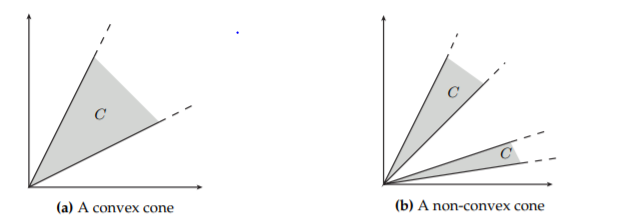
\includegraphics[width=0.8\textwidth]{cones.png}
	\caption{Cones}
\end{figure}

From the illustration we can conclude, that:
\begin{itemize}
	\item $\exists c=\lambda a + (1-\lambda)b: z \not\in K_{\text{non-convex}}, a,b \in K$
	\item $\nexists c=\lambda a + (1-\lambda)b: z \not\in K_{\text{convex}}, a,b \in K$
\end{itemize}
	Since there exists $z = x + y$ and $z$ goes through the point $c$, $z \in K$ if and only if $K$ is convex.
	\item Each convex cone has at most one extreme point, namely the origin.

	If there more than one extreme point in a cone (convex is not necessary), than \newline$E\lambda\geq 0: \lambda x \not\in C, x \in C$, which contradicts the definition.
	\item A polyhedral cone of the form $K:={x\in \R^n|Ax\leq 0} (\text{ with }A\in \R^{m\times x})$ has exactly one extreme point, namely the origin.

From my point of view it's the same as b.
\end{enumerate}
\exercise
Let us represent each individual interval as a function:
\begin{align*}
	&f_{1, 1} = 3520.20 + 51.20x_{1,1} \\
	&f_{2, 1} = 82810.00 + 52.10x_{2,1} \\
	&f_{2, 2} = 82810.00 + 52.10\cdot 20000 + 51.10x_{2,2} \\
	&f_{2, 3} = 82810.00 + 52.10\cdot 20000 + 51.10\cdot40000 + 50.10x_{2,3} \\
	&f_{2, 4} = 82810.00 + 52.10\cdot 20000 + 51.10\cdot40000 + 50.10\cdot20000 + 49.10x_{2,4} \\
	&f_{3, 1} = 60.50x_{3,1} \\
	&f_{3, 2} = 60.50\cdot50000 + 59.00x_{3,2}, 
\end{align*} 
where $x_{i,j}$ - count of goods in $i,j$-interval. \newline Also, let us associate with each $i,j$ - interval a binary variable $y_{i,j}$ such
that, $y_{i,j} = 1$ if $i,j$ - interval is chosen, else $y_{i,j} = 0$.

Hence, the corresponding optimization problem:
\begin{align*}
	\text{min} \quad
	&y_{1,1}f_{1, 1} + y_{2,1}f_{2, 1}+ y_{2,2}f_{2, 2}+ y_{2,3}f_{2, 3}+ y_{2,4}f_{2, 4}+ y_{3,1}f_{3, 1}+ y_{3,2}f_{3, 2}+x_{1,1} +x_{2,2}+x_{2,3}+x_{2,4}+x_{3,1}+x_{3,2} \\
	\text{s.t.} \quad
	&y_{1,1}x_{1,1}+\\ 
	&y_{2,1}x_{2,1}+ y_{2,2}(20000+x_{2,2})+y_{2,3}(60000+x_{2,3})+y_{2,4}(80000+x_{2,4})+\\
	&y_{3,1}x_{3,1}+y_{3,2}(50000+x_{3,2}) = 150000 \\
	&y_{1,1}\leq1 \\
	&y_{2,1} +y_{2,2} +y_{2,3} +y_{2,4}\leq1 \\
	&y_{3,1} +y_{3,2}\leq1 \\
	&x_{1,1} \leq 50000 \\
	&x_{2,1} \leq 20000 \\
	&x_{2,2} \leq 40000 \\
	&x_{2,3} \leq 20000 \\
	&x_{2,4} \leq 20000 \\
	&x_{3,1} \leq 50000 \\
	&x_{3,2} \leq 30000 \\
	&x_{1,1},x_{2,2},x_{2,3},x_{2,4},x_{3,1},x_{3,2} \geq 0 \\
	&y_{1,1},y_{2,2},y_{2,3},y_{2,4},y_{3,1},y_{3,2} \in \{0, 1\} \\
	&x_{1,1},x_{2,2},x_{2,3},x_{2,4},x_{3,1},x_{3,2} \in \Z
\end{align*}
We added $x_{1,1} +x_{2,2}+x_{2,3}+x_{2,4}+x_{3,1}+x_{3,2}$ in an objective function in order to fix such problem: if $y_{2,1} = 1$ and $y_{2,2} = 0$ then $x_{2,2}$ can be any value $\geq 0$, but for this objective function $x_{2,2}$ will be equal to zero.

The objective function is twice differentiable. Hence, we can examine Hessian. It's obvious that Hessian matrix is a positive semidefinite $\Rightarrow$ the objective function is convex.Since, each constraint is a convex function, covex set is also convex.
\exercise
Consider the polyhedron $P$, which is given by the following five inequalities: \[x_1 + 2x_2\geq 1, -x_1\leq 1, x_1 - x_2 \geq -3, x_2\geq 1, -2x_1-x_2\leq0\]
\begin{enumerate}[label=(\alph*)]
	\item Make a drawing of the polyhedron $P$.
	\begin{center}
	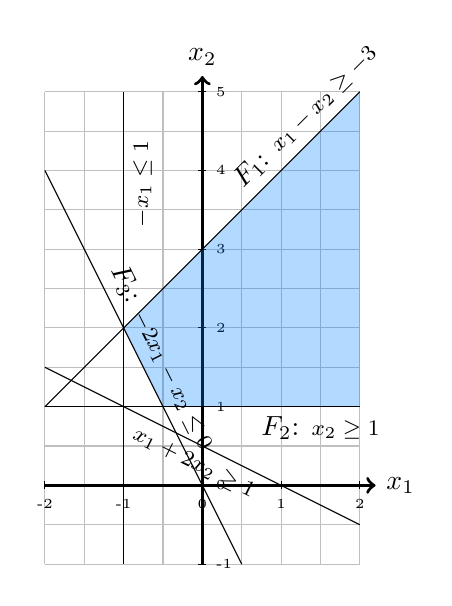
\begin{tikzpicture}
	
	    \draw[gray!50, thin, step=0.5] (-2,-1) grid (2,5);
	    \draw[very thick,->] (-2,0) -- (2.2,0) node[right] {$x_1$};
	    \draw[very thick,->] (0,-1) -- (0,5.2) node[above] {$x_2$};
	
	    \foreach \x in {-2,...,2} \draw (\x,0.05) -- (\x,-0.05) node[below] {\tiny\x};
	    \foreach \y in {-1,...,5} \draw (-0.05,\y) -- (0.05,\y) node[right] {\tiny\y};
	
	    \fill[blue!50!cyan,opacity=0.3] (2,5) -- (-1,2) -- (-0.5,1) -- (2,1) -- cycle;
	
	    \draw (-2,1.5) -- node[below,sloped] {\footnotesize$x_1+2x_2\geq1$} (2,-0.5);
	    \draw (-1,-1) -- (-1, 4) -- node[below left,sloped] {\footnotesize$-x_1\leq1$} (-1,5);
	    \draw (-2,1) -- (1,4) -- node[above,sloped] {$F_1$: \footnotesize$x_1-x_2\geq-3$} (2,5);
	    \draw (-2,1) -- (1,1) -- node[below,sloped] {$F_2$: \footnotesize$ x_2\geq1$} (2,1);
	    \draw (-2,4) -- node[above,sloped] {$F_3$: \footnotesize$-2x_1-x_2\leq0$} (0.5,-1);
	
	\end{tikzpicture}
	\end{center}
	\item Determine at the hand of your drawing all faces of the polyhedron and state a defining inequaliti for each face.
	\begin{align*}
	F_1 = P\cap\{x\in \R^2: x_1 - x_2 \geq -3\} \\
	F_2 = P\cap\{x\in \R^2: x_2 \geq 1\} \\
	F_3 = P\cap\{x\in \R^2: -2x_1 - x_2 \leq 0\}
	\end{align*}
	\item State at the hand of your drawing a matrix $A$ and a vector $b$ such that both $P=P(A,b)$ holds and the system $Ax\leq b$ is irredundant.
	\[ A =
	\begin{pmatrix}
	-1 & 1\\
	0 & -1 \\
	-2 & -1
	\end{pmatrix}
	, b =
	\begin{pmatrix}
	3\\
	-1\\
	0
	\end{pmatrix}
	\]
	\item Find a matrix $B$ and a vector $c$ such that $P$ is eqivalent to $P^=(B,c)$. Is $P=P^=(B,c)$?

	By definition: $P^=(B,c)\coloneqq\{x:Bx=c,x\geq0\}$. Let $x_i = x_i^+ - x_i^-\text{ where }x_i^+, x_i^- \geq0$ and $y_1, y_2, y_3$ are slack variables, , then the system of inequalities can be written as an equivalent system of equalities:
	\[ B =
	\begin{pmatrix}
	-1 & 1 & 1 & -1 & 1 &0 &0\\
	0 & 0 &-1 & 1 & 0 &1 &0 \\
	-2 & 2 & -1 & 1 &0 &0 &1
	\end{pmatrix}
	, c =
	\begin{pmatrix}
	3\\
	-1\\
	0
	\end{pmatrix}
	\], where $x = (x_1^+ , x_1^-, x_2^+ , x_2^-, y_1, y_2, y_3)^T$. Hence, $P^=(B,c)=\{x\in R^7: Bx=c, x\geq0\}$.
\end{enumerate}
\textbf{P.S. It would be great if you provide a solution where it is wrong.}
\end{document}